\documentclass[12pt, notitlepage, final]{article} 

\newcommand{\name}{Vince Coghlan}

%\usepackage[dvips]{graphics,color}
\usepackage{amsfonts}
\usepackage{amssymb}
\usepackage{amsmath}
\usepackage{latexsym}
\usepackage{enumerate}
\usepackage{amsthm}
%\usepackage{nccmath}
\usepackage{setspace}
\usepackage[pdftex]{graphicx}
\usepackage{epstopdf}
%\usepackage[siunitx]{circuitikz}
\usepackage{tikz}
\usepackage{float}
%\usepackage{cancel} 
\usepackage{setspace}
%\usepackage{overpic}
\usepackage{mathtools}
\usepackage{listings}
\usepackage{color}
%\usepackage{gensymb}

\numberwithin{equation}{section}
\DeclareRobustCommand{\beginProtected}[1]{\begin{#1}}
\DeclareRobustCommand{\endProtected}[1]{\end{#1}}
\newcommand{\dbr}[1]{d_{\mbox{#1BR}}}
\newtheorem{lemma}{Lemma}
\newtheorem*{corollary}{Corollary}
\newtheorem{theorem}{Theorem}
\newtheorem{proposition}{Proposition}
\theoremstyle{definition}
\newtheorem{define}{Definition}
\newcommand{\column}[2]{
\left( \begin{array}{ccc}
#1 \\
#2
\end{array} \right)}

\newdimen\digitwidth
\settowidth\digitwidth{0}
\def~{\hspace{\digitwidth}}

\setlength{\parskip}{1pc}
\setlength{\parindent}{0pt}
\setlength{\topmargin}{-3pc}
\setlength{\textheight}{9.0in}
\setlength{\oddsidemargin}{0pc}
\setlength{\evensidemargin}{0pc}
\setlength{\textwidth}{6.5in}
\newcommand{\answer}[1]{\newpage\noindent\framebox{\vbox{{\bf ECEN 3400 Spring 2014} 
\hfill {\bf \name} \vspace{-1cm}
\begin{center}{Homework \#1}\end{center} } }\bigskip }

%absolute value code
\DeclarePairedDelimiter\abs{\lvert}{\rvert}%
\DeclarePairedDelimiter\norm{\lVert}{\rVert}
\makeatletter
\let\oldabs\abs
\def\abs{\@ifstar{\oldabs}{\oldabs*}}
%
\let\oldnorm\norm
\def\norm{\@ifstar{\oldnorm}{\oldnorm*}}
\makeatother

\def\dbar{{\mathchar'26\mkern-12mu d}}
\def \Frac{\displaystyle\frac}
\def \Sum{\displaystyle\sum}
\def \Int{\displaystyle\int}
\def \Prod{\displaystyle\prod}
%\def \P[x]{\Frac{\partial}{\partial x}}
%\def \D[x]{\Frac{d}{dx}}
\newcommand{\PD}[2]{\frac{\partial#1}{\partial#2}}
\newcommand{\PF}[1]{\frac{\partial}{\partial#1}}
\newcommand{\DD}[2]{\frac{d#1}{d#2}}
\newcommand{\DF}[1]{\frac{d}{d#1}}
\newcommand{\fix}[2]{\left(#1\right)_#2}
\newcommand{\ket}[1]{|#1\rangle}
\newcommand{\bra}[1]{\langle#1|}
\newcommand{\braket}[2]{\langle #1 | #2 \rangle}
\newcommand{\bopk}[3]{\langle #1 | #2 | #3 \rangle}
\newcommand{\Choose}[2]{\displaystyle {#1 \choose #2}}
\newcommand{\proj}[1]{\ket{#1}\bra{#1}}
\def\del{\vec{\nabla}}
\newcommand{\avg}[1]{\langle#1\rangle}
\newcommand{\piecewise}[4]{\left\{\beginProtected{array}{rl}#1&:#2\\#3&:#4\endProtected{array}\right.}
\newcommand{\systeme}[2]{\left\{\beginProtected{array}{rl}#1\\#2\endProtected{array}\right.}
\def \KE{K\!E}
\def\Godel{G$\ddot{\mbox{o}}$del}

\onehalfspacing

\begin{document}

\answer{}

1) \textbf{P1.9:}
\begin{figure}[H]
\begin{center}
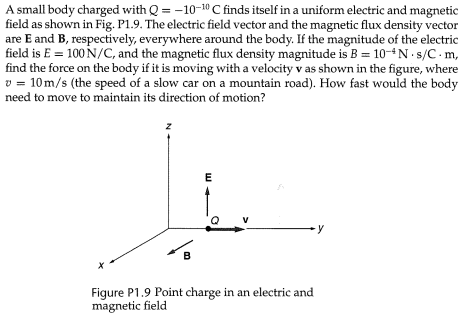
\includegraphics[width=12cm]{f1}
\end{center}
\end{figure}
To find the force we can use two simple equations:
\[
\bar{F_m} = Q\bar{v} \times \bar{B} \text{ and } \bar{F_e} = \bar{E}\cdot q
\]
We can work these out:
\[
\bar{F_m} = -10^{-10} \cdot (10 \cdot 10^{-4})(-\hat{z}) = 10^{-13}\hat{z}
\]
\[
\bar{F_e} = 100 \cdot -10^{-10} (\hat{z}) = -10^{-8}\hat{z}
\]
The vectors are in opposite directions and thus the force felt by the charged body is mostly from the electric field, which would be: $\bar{F} \approx -10^{-8}\hat{z}$. In order for the object to maintain its direction:
\[
|\bar{F_m}| = |\bar{F_e}| \Rightarrow -10^{-10} \cdot (v \cdot 10^{-4})= 100 \cdot -10^{-10} \Rightarrow v = 1\cdot 10^6 \;\text{m/s}
\]
\newpage

2) \textbf{P2.1:}
\begin{figure}[H]
\begin{center}
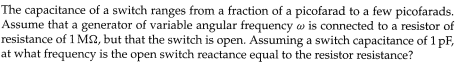
\includegraphics[width=12cm]{f2}
\end{center}
\end{figure}

The resistance of a capacitor is $\frac{1}{C\omega}$, we can setup a simple equation to solve this problem:
\[
\frac{1}{1 \cdot 10^{-12}\cdot \omega} = 1\cdot 10^6 \Rightarrow \omega = 1\;\text{MHz}
\]

3) A surface-mount chip capacitor package has an unknown parasitic inductance $L$. You need to use the capacitor at some high frequency and therefore you need to find out what $L$ is, i.e. is the capacitor starting to act as an inductor at your design frequency. To find the parasitic inductance, which is assumed to be the same for all capacitors with the same package, you can do the following experiment: order several capacitors of different values - 1pF, 40pF, 80pF. Then connect each to ground and measure the input impedance as a function of frequency. The measurement shows resonant frequencies of 1.01, 1.44 and 8.001GHz (how do you know what the resonant frequency is from an impedance measurement?). What is your best estimate of the parasitic inductance of this surface-mount package? What is your estimate on the tolerance in the value of the spec-sheet capacitance?\\

The resonant frequency of a $LC$ circuit is $\frac{1}{2\pi\sqrt{LC}}$, thus we can solve for $L$.
\[
1.01 \cdot 10^9 = \frac{1}{2\pi\sqrt{L \cdot 1 \cdot 10^{-12}}} \Rightarrow L = 2.48 \cdot 10^{-8} L
\]
\[
1.44 \cdot 10^9 = \frac{1}{2\pi\sqrt{L \cdot 40 \cdot 10^{-12}}} \Rightarrow L = 3.05 \cdot 10^{-10} L
\]
\[
8.001 \cdot 10^9 = \frac{1}{2\pi\sqrt{L \cdot 80 \cdot 10^{-12}}} \Rightarrow L = 4.95 \cdot 10^{-12} L
\]
My estimate for the parasitic inductance will be right in the middle, at 300pH.  The tolerance on the capacitance is probably maximized at 80 pF when we use this parasitic inductance.  We find it to be $\pm 1.3$pF, this is $\pm1.6\%$.

\newpage

4) \textbf{P3.14:}
\begin{figure}[H]
\begin{center}
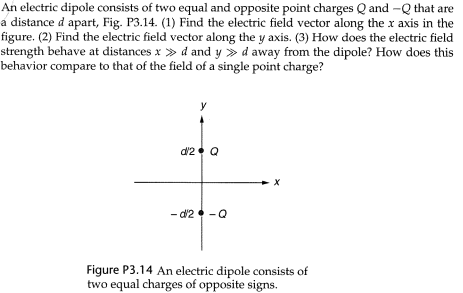
\includegraphics[width=12cm]{f3}
\end{center}
\end{figure}

(1) The electric field vector along the x axis will be in the $-y$ direction along the entire axis.  The magnitude can be found like so:
\[
\bar{E} = -\frac{kQ}{x^2 + (\frac{d}{2})^2}\hat{y}
\] 

(2) Along the y axis it varies.  For $\frac{-d}{2}>y>\frac{d}{2}$ then the force points in the positive direction.  The field would be the sum of the two fields from the charges:
\[
\bar{E} = (\frac{kQ}{(y - d/2)^2} - \frac{kQ}{(y + d/2)^2})\hat{y}
\]

(3) As $x >> d$ and $y >> d$ then the two charges begin to behave as one, and the field from each charge cancels out.  This is not true of a single point charge, where the force would be much stronger at that distance.


\newpage

5) \textbf{P3.23:}
\begin{figure}[H]
\begin{center}
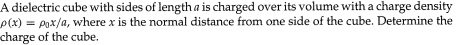
\includegraphics[width=12cm]{f4}
\end{center}
\end{figure}

This is a geometry problem:
\[
\int_V p(x) dV = \int_0^a \int_0^a \int_0^a p_0\frac{x}{a}dxdydz = p_0\frac{a^3}{2}
\]

6) \textbf{P4.5:}
\begin{figure}[H]
\begin{center}
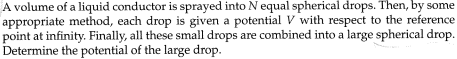
\includegraphics[width=12cm]{f5}
\end{center}
\end{figure}
The potential of all the drops together would be $N\cdot V$. This is because the voltage from infinity will be defined as:
\[
V_A = \frac{Q}{4\pi\epsilon_0r}
\]
And since the the radius and constant don't change, each drop has a measurable charge.  When we put the drops together the charge adds on itself, and we are left with more charge.  $N$ drops means:
\[
V_{A\;\text{new}} = \frac{k\cdot N\cdot Q}{r} = N\cdot V_A
\]

\newpage

7) \textbf{P4.12:}
\begin{figure}[H]
\begin{center}
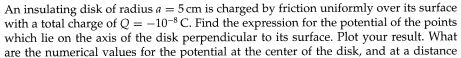
\includegraphics[width=12cm]{f6}
\end{center}
\end{figure}
\begin{figure}[H]
\begin{center}
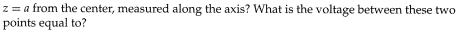
\includegraphics[width=12cm]{f7}
\end{center}
\end{figure}

The potential equation can be found using an integral:
\[
V = \int_A \frac{k\cdot Q}{R} dA
\]
The nifty way of doing this problem is in radial coordinates(adding up a bunch of charged rings).  If the area is $5$cm and we know the charge, then the charge density is $-1.273 \cdot 10^{-6}$ C/m.  The charge on any one of the rings $dq = \sigma(2\pi r dr)$.  The potential from a ring is:
\[
dV = k\frac{dq}{\sqrt{z^2 + r^2}} = 2\pi\sigma k\frac{rdr}{\sqrt{z^2 + r^2}}
\]
We can now add these up:
\[
V(z) = 2\pi\sigma k \int_0^{.05} \frac{rdr}{\sqrt{z^2 + r^2}} = 2\pi\sigma k (\sqrt{z^2 + (0.05)^2} - z)
\]
This looks like:
\begin{figure}[H]
\begin{center}
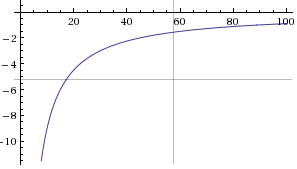
\includegraphics[width=8cm]{f8}
\end{center}
\end{figure}
For $z = a$:
\[
V = 2\pi\sigma k (\sqrt{a^2 + (0.05)^2} - a)
\]






















\end{document}